\documentclass{udparticle}
\setlogo{EIT}
\headertext{Respuestas tarea de preparación para la Solemne }
\title{Tarea de preparación para la Solemne 2}
\author{Ignacio Yanjari, Dagoberto Navarrete, Ignacio López, Thomas Muñoz.}
\usepackage{graphicx}
\usepackage{float}
\graphicspath{ {images/} }
\begin{document}
\maketitle
\begin{enumerate}
%\clearpage
\item Nombre 3 servicios ofrecidos por la Capa de RED.

\begin{enumerate}
	\item Permite la conexión entre 2 redes geograficamente distintas
	\item Busca la mejor ruta desde una red a otra mediante criterios
	\item Utiliza un sistema de correccion de errores al transportar paquetes
\end{enumerate}

\item Explique brevemente las causas que gatillaron el problema de escases de las direcciones IPv4.\\
Como solo existian Clases de IPs con mascaras por defecto para c/clase,generaba una 
perdida de muchas combinaciones de ip al momento de asignarle una clase a una casa por 
ejemplo.\\
Mecanismos para mitigar problemática:

\begin{enumerate}
	\item Tecnica de sumarizacion de redes 
	\item Tecnica de  creacion de subredes
	\item Ip privada y Ip pública
\end{enumerate}

\item Realice una breve descripción de cada uno de los campos de la cabecera IPv4. Se pide utilizar la aplicacion Wireshark para realizar 1 captura (pantallazo) e interpretar la información relacionada con la capa de red (todos los campos de la cabecera IPv4).
\item Explique las diferencias existentes entre el protocolo IPv4 e IPv6.
\item El prefijo de una red IPv6 es: 2001:0720:1014:0002. Se conecta un
computador cuya dirección física MAC es 0008:0267:5CCA. Se pide indicar la direccion IPv6 del equipo.
\item ¿Cual es la unidad máxima de transferencia MTU para una red Ethernet?
\item Indique la dirección resumida de la IPv6 0004:0000:0000:0000:000A:0000:0000:1243:00AD
\item Explique las diferencias existentes entre los modos túnel, traductor y dual stack
\item Se pide realizar la conversión binaria a decimal de la información contenida en la tabla Figura 1.
	\begin{figure}[H]
	\centering
	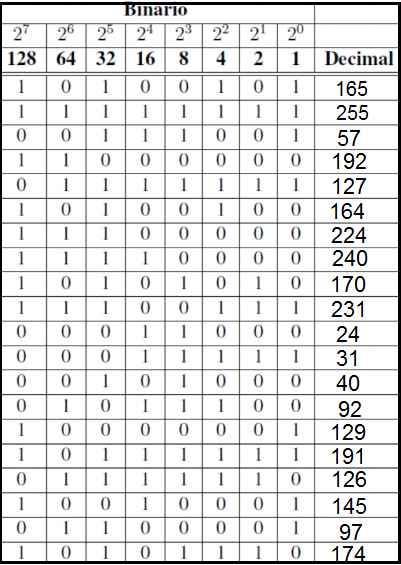
\includegraphics[width=15cm]{fig1}
	\caption{Cálculo de binario a decimal}
	\end{figure}
\clearpage

\item Se pide realizar la conversion de decimal a binario de la información contenida en la tabla de la Figura 2.
	\begin{figure}[H]
	\centering
	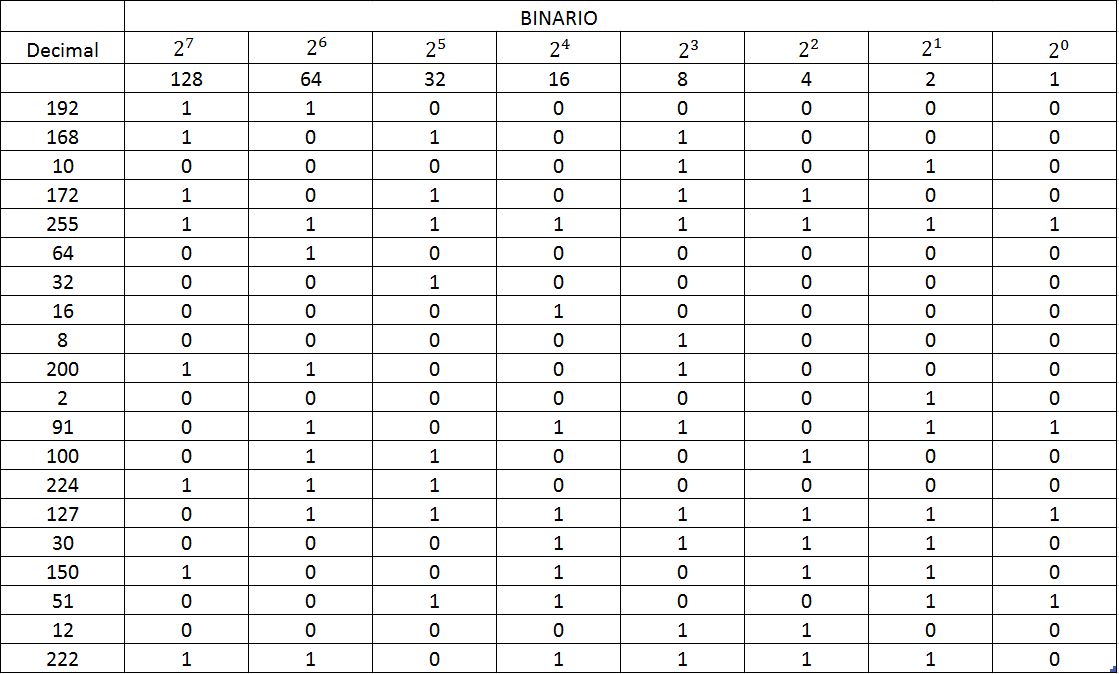
\includegraphics[width=15cm]{fig2}
	\caption{Cálculo de decimal a binario}
	\end{figure}

%insertar figura 2
\item Indique la importancia del uso de NAT/PAT.
Permite el uso de ip privadas y publicas.Siendo privadas las que se encuentran en la LAN y las ip pública es la
salida de esta LAN recien mencionada a la WAN.Generando asi menor cantidad de ips en uso ya que pueden existir
2 ips iguales pero dentro de difentes LAN.\\
\item ¿Que es NAT? ¿Qué es PAT?
Son tipos de traducciones dentro de un router :
\begin{enumerate}
	\item NAT : genera la asociación entre una IP pública y una IP privada dentro de la red
	\item PAT : genera la asociación entre una Ip pública con su respectivo puerto en el router
\end{enumerate}
\item Explique las diferencias entre NAT estática y NAT dinámica.
\begin{enumerate}
\item NAT estática es una traducción sin cambios automáticos,dejando a el administrador como
el que configure la tabla.Esto se aplica principalmente para dispositivos que como requerimiento
necesiten una IP estática,por ejemplo Servidor WEB.Si se quisieran agregar más servidores se tendrían que 
configurar todos manualmente.\\
\item NAT dinámica es una traducción en la cual cuando se agrega un dispositivo en la LAN, automáticamente
se configura la tabla sin necesidad de un administrador.Se usa para host como PC,ya que estos pueden utilizar
IP dinámica y así se facilitaria la conección de una gran cantidad de dispositivos.\\
\end{enumerate}
\item Un router que hace la siguiente NAT dinamica: red interior 
192.168.0.0/24 <-> red exterior 200.230.16.192/26.\\
¿Cual es el rango de direcciones IPs pública con los que los equipos 
pueden salir?
\item ¿Que es una ACL estándar?\\\\
Una ACL es una lista de control de acceso permitida en los routers,el tipo estándar permite filtrar antes o despues 
de pasar por el router pero solo se puede filtrar según IP origen.ubicando en la wild-card el 0 indica el valor estático 
y 1 el variable.\\
por ejemplo:
\begin{enumerate}
\item para filtrar un solo usuario de ip 192.13.13.1 se ocuparia la wild-card igual a 0.0.0.0
\item para filtrar una red de ip 192.13.13.0 se le aplicaría la wild-card igual a 0.0.0.255
\end{enumerate}
sintaxis 'Router (config-if)# ip access-group nº in|out"
\item ¿Que es una ACL extendida?\\\\
Una ACL es una lista de control de acceso permitida en los routers,el tipo extendida permite filtrar antes o despues
dependiendo de el protocolo(IP, ICMP, TCP, UDP, ...)tendremos opciones de configuración diferente, siempre acorde con 
el protocolo, es decir con TCP podré utilizar operación de puertos pero con IP no.
sintaxis 'Router (config)# access-list nº permit|deny protocolo origen [wild-mask] [operación] [puerto origen] destino [wild-mask] 
[operación] [puerto destino] [established]"
\item La empresa ACME SA tiene una red como la que muestra la Figura 3. 
En el router R0 se han establecido 2 ACLs. La primera ACL tiene por 
objetivo de filtrar el tráfico de entrada hacia el 
servidor DMZ con las siguientes reglas:\\
Regla1 > permit tcp any any\\
Regla2 > permit udp any any\\
Regla3 > permit ip any any\\
Regla4 > permit icmp any any\\
La segunda ACL filtra el trafico de entrada hacia la red 
192.168.1.0/24:\\
Regla1 > deny tcp any 192.168.1.200\\
Regla2 > permit tcp any any\\
Regla3 > permit ip any 192.168.1.200\\
Regla4 > permit ip any any\\
Explique la funcion que cumple cada una de estas reglas.\\
\item Implemente los filtros necesarios para controlar los posibles ataques a los equipos de la red ACME, excepto los que corresponden
a los servicios web y ftp que se encuentran alojados en el servidor 192.168.1.200.

\item ¿Que es una subred?.
Es una division de una red cuando estás son muy grandes.Sirve para reducir el dominio broadcast y obtener un mayor manejo dentro
de la red.
\item De la direccion de red 136.228.0.0 se han de generar 99 subredes de igual tamaño.¿Cuál es la máscara que se debe utilizar?.
\item Para la misma red del caso anterior, indique la cantidad máxima de hosts que por cada una de las subredes
\item Si se tiene un host cuya direccion IP y prefijo son: 19.95.99.210 
/25.Indique su dirección de red.
su dirección de red es 19.95.99.0/25
\item Si una red Clase C se divide en subredes cuya mascara es 255.255.255.192, ¿Cuántas subredes utilizables se crean?.
\item Dada una dirección IP de host 192.168.5.121 y una máscara de 
subred 255.255.255.248, ¿Cuál es el numero IP de la red del host?.
\item ¿En que se diferencian las direcciones de MAC de las de la capa de red?.
\item ¿Cuantas direcciones útiles de host se pueden utilizar en una red con prefijo 24?.
\item ¿Cuantas subredes pueden tener una red que tiene un prefijo 16?.
\item ¿Cual es el número mínimo de bits que se pueden tomar prestados para formar una subred?.
\item ¿Cuales son las principales razones para utilizar subredes?.
\item Al realizar una operacion booleana en las direcciones IP 131.8.2.5
AND 255.0.0.0 como lo haría un router, ¿Cuál sería la dirección de 
red/subred?.
\item Con una direccion de Clase C de 197.15.22.31 y una máscara de red 
de 255.255.255.224,¿cuántos bits se tienen que tomar prestados para 
crear subredes?.
\item Si usted quiere tener 12 subredes de Clase C, ¿cual es la máscara 
a utilizar?.
\item Si usted necesita una red de prefijo 16 y desea generar 510 
direcciones de subredes, ¿cuál es la máscara que se deber ıa utilizar?.
\item De la topología de red, mostrada en la Figura 4, se deben generar 
las subredes solicitadas, para esto usted debe utilizar la tecnica de 
longitud de máscara variable VLSM de tal forma de maximizar el espacio 
de direcciones IPs. Se dispone de la dirección 192.200.254.0/23 la cual 
usted debe utilizar para generar las subredes. Se pide completar la 
tabla de la Figura 5. Nota: las direcciones IP de las interfaces Fast 
Ethernet de todos los routers NO están consideradas en los requerimientos.
%Insertar Figura 4
\item Usted, como especialista en el diseno de redes LAN, ha sido seleccionado para
finalizar el proyecto que se muestra en la Figura 6. El ISP le ha asignado 2 
direcciones IP publicas: la dirección 177.12.180.252/30, que será utilizada como 
enlace con el ISP, y la dirección 200.198.248.0/21 la cual debe utilizar para 
generar las subredes necesarias mediante la técnica de máscara variable VLSM.
Se pide completar el diagrama de red (Figura 6) con la informacion solicitada
(direcciones de sub-redes, máscaras, dirección de broadcast, dirección IP 
hosts, gateway y enlaces seriales).
%Insertar figura 5/6
%REVISAR IMAGEN 5 o 6 respecto a la pregunta anterior
\clearpage
\item Una organizacion se divide en dos departamentos A y B. La red corporativa de 
dicha organización se divide, a su vez, en cinco subredes tal y como muestra la 
Figura 7. Para ello, la organizacion dispone de la dirección de red 138.8.0.0. 
Las subredes A1, A2 y A3 pertenecen al departamento A, y las subredes B1 y B2 
pertenecen al departamento B. Dicha red corporativa se conecta a Internet    a traves 
del router 3.\\
a) ¿Que máscara de red se debe utilizar en cada una de las redes en que se ha   
dividido la red corporativa original, si se desea que quede asignable en cada una 
de dichas redes el mayor numero posible de direcciones IP?\\

b)¿Cual es el máximo número de direcciones IP asignables a cada una de las subredes?\\

c)¿Que dirección IP destino debe utilizar un equipo perteneciente a la subred B2 si
desea transferir un paquete IP a todos los equipos de la red A2?\\

d)¿Podría transferir, un equipo perteneciente a la subred B1, un paquete IP a todos
los equipos del departamento A?. En caso de que la respuesta sea afirmativa,
indique que dirección IP de destino se debe utilizar\\

%Insertar figura 7

\item De la topología de red de la Figura 8, complete la tabla de rutas del 
Router/Firewall. Indique si es posible realizar una sumarización de la tabla de 
rutas anterior (justifique). Si su respuesta es afirmativa se pide construir esta tabla de rutas resumida.
%insertar figura 8

\item Dada la siguiente topología de la Figura 9, encontrar la tabla de rutas del 
router R1. También se pide encontrar la tabla de ruta sumarizada. En ambos casos 
considere la existencia de una ruta por defecto.
%insertar figura 9

\item Se tiene la siguiente tabla (Figura 10) de enrutamiento sin CIDR. Encuentre 
la tabla del router reducida utilizando sumarizacion CIDR.
%Insertar figura 10
\item En la red de la Figura 11 las redes Ethernet conectadas a R1 han sido 
notificadas de manera sumarizada hacia R2 como 192.168.144.0/20. ¿Cuáles serán 
las direcciones IP de los paquetes que se enviara el router R2 hacia R1, de acuerdo a este resumen?.
%Insertar figura 11
\item Para la red de la Figura 12, determine, ¿cuál es la mejor ruta sumarizada que
enviará R3 a R4?. 
%Insertar figura 12

\item Para la red de la Figura 13, determine si el usuario de notebook del 
departamento de VENTAS de la SUCURSAL 1 puede o no puede comunicarse con el Server 
A del departamento de MARKETING,ubicado en la CASA MATRIZ. Si su respuesta es 
negativa, indique cómo resolver el problema.
%Insertar figura 13

\item Después de ser instalada y configurada la red de la Figura 14, se ha 
comprobado que ésta no funciona correctamente. Usted, como especialista, ha sido 
contratado para resolver el problema. Identifique el problema y proponga el o los 
cambios que se deben realizar.
%Insertar figura 14

\item ¿Que es un sistema autónomo AS y qué representa un ASN?.
\item Explique las diferencias existentes entre los protocolos de ruteo basado en
vector-distancia (algoritmo de Bellman-Ford) y estado de enlace (algoritmo de Dijkstra).

\item ¿Que métrica utiliza RIP para determinar la mejor ruta?.
\item ¿Que significa una distancia administrativa de 255?.
\item Una tabla de enrutamiento muestra la información: S* 0.0.0.0/0 [1/0] via 172.16.10.5. ¿Qué significa?
\item Señale ventajas y desventajas del enrutamiento estático. Cite dos ejemplos donde convenga usarlo.
\item Complete la Tabla (Figura 15) escribiendo Si o No en cada celda segun corresponda.
%figura 15

\item Indique cuales de los siguientes protocolos de enrutamiento permiten VLSM y 
cuáles no: RIP v1; RIP v2; EIGRP; OSPF
\item Indique cuáles de los siguientes protocolos admiten enrutamiento sin clase y 
cuáles no: IGRP,EIGRP, RIP v1, RIP v2, OSPF, IS-IS. ¿Cuáles son de vector 
distancia? ¿Cuáles de estado de enlace?
\item Senale cuál(es) métrica(s) usan los siguientes protocolos de enrutamiento de gateway interior:RIP, EIGRP, OSPF.
\item ¿Qué es la distancia administrativa en un protocolo de enrutamiento?
\item ¿Cuáles son las distancias administrativas para: redes directamente conectadas, rutas estáticas,RIPv1, RIPv2, EIGRP interno, EIGRP externo, OSPF?
\item Cite un ejemplo donde la distancia administrativa sea el determinante en la decisión de enrutamiento.
\item Un router corporativo recibe un paquete IP con direccion origen 
192.168.214.20 y dirección destino 192.168.22.3. Determine qué hará el router con este paquete si su tabla de enrutamiento muestra la siguiente información: ´
RouterUDP> show ip route [?]\\
R 192.168.215.0 [120/2] via 192.168.20.2 00:00:23, Serial 0/0/0\\
R 192.168.115.0 [120/1] via 192.168.20.2 00:00:23, Serial 0/0/0\\
R 192.168.30.0 [120/2] via 192.168.20.2 00:00:23, Serial 0/0\\
C 192.168.20.0 is directly connected, Serial 0/0/0\\
C 192.168.214.0 is directly connected, Serial 0/0/0, FastEthernet 0/0\\

\item ¿Cual es el propósito del área 0 en OSPF?
\item ¿Cual es el propósito de emplear interfaz de loopback con máscara 255.255.255.255 en OSPF?
\item Los routers de la Figura 16 se encuentra ejecutando OSPF en el area 0. 
Determine cuál será el router ID por defecto publicado por el router CONCEPCION.
%insertar figura 16
\item Nombre 3 servicios ofrecidos por la capa de Transporte.
\item Explique las diferencias existentes entre los protocolos de transporte TCP y UDP
\item ¿ Cual es la ventaja del protocolo UDP sobre TCP?
\item ¿Qué usan UDP y TCP para registrar las distintas conversaciones que cruzan una red al mismo tiempo?.
\item ¿Cual es el propósito de los números de puertos?. ¿Cuáles son tipos y rangos de direcciones IP?
\item ¿Cuál es el comando que nos permite conocer las conexiones abiertas?. 
¿Cuál es el comando que muestra los puertos en estado de escucha?
\item ¿Para qué se utiliza el saludo de tres vías en TCP?.
\item ¿Cual es la función de una ventana deslizante en TCP?
\item ¿Qué indica el campo Ventana en un segmento TCP?.
\item ¿Cómo sincroniza TCP una conexión entre el origen y el destino antes de la 
transmisión de datos?.
\item En una transmision TCP, ¿qué ocurre si un segmento no es confirmado tras un 
determinado periodo de tiempo?.
\item Explique los mecanismos utilizados para realizar el control de congestion y control de flujo.
\item Explique a traves de las primitivas el establecimiento de una conexión del
tipo socket TCP entre un equipo cliente y un servidor.
\item Explique en que consiste el mecanismo de control de congestión en TCP denominado partida lenta.
\item Explique en qué consiste el problema del síndrome de la ventana tonta y cual es la solución a este problema.


\end{enumerate}
\end{document}
